% nodo geth in ascolto sulla rete di due console 


\section{L'applicazione}\label{ssec:Progettazione}
	Lo scopo della seguente ricerca è l'implementazione di un'applicativo finalizzato alla gestione delle opere autoriali. Esso consente la registrazione, la visione di opere autoriali e la classifica delle stesse in base all'utilizzo reale degli utenti. Il sistema sarà implementato mediante smart contract in esecuzione sulla piattaforma Ethereum, ciò consentirà di disporre delle proprietà di trasparenza, tracciabilità e immutabilità proprie della blockchain.\\
	
	Verrà utilizzata la seguente terminologia:
	\begin{description}
		\item[Utente] o account: è la persona che sottoscrive la registrazione di un opera (proprietario) o acquista il diritto all'utilizzo di una determinata opera(compratore).
		\item[Opera]: è l'opera creativa, identificata tramite i metadati che il proprietario inserisce in fase di registrazione.
		\item[Contratto di registrazione] o registrazione: rappresenta la prova verificabile della cessione del diritto di utilizzo dell'opera.
		\item[Digichain] o libro mastro o ledger: è l'entità decentralizzata che gestisce l'interazione tra le componenti, è unico e da esso è possibile esercitare tutte le operazioni permesse.
	\end{description}
	
	Anche se lo sviluppo di smart contract si è concentrato sull'applicazione \textit{Digichain}, sono stati sviluppati altri contratti tra cui \textit{GlobalRegistrar} che consente di condividere in modo immediato un indirizzo tramite un nome simbolico. Questo permette di non dover più comunicare l'indirizzo di un contratto mediante sistemi esterni alla blockchain, ma più semplicemente sfruttare il concetto di database e smart contract per implementare un ente di registrazione. 
	
	\subsection{Registrar}
	
	In Ethereum ogni account, che sia uno smart contract o un utente esterno, viene identificato mediante indirizzo univoco a 160bit. Quando un utente vuole spedire un certo ammontare di Ether o vuole eseguire una chiamata ad un contratto deve recuperare in tutti e due i casi l'indirizzo del destinatario e, solo nell'ultimo, deve reperire l'abi del contratto\footnote{Riferirsi al capitolo \ref{sssec:sviluppareinsolidity}}. Per l'ultimo caso, visto che è alquanto dispendioso l'inserimento nella blockchain dell'intera interfaccia delle chiamate del contratto, nella main-chain di Ethereum l'abi viene fornito tramite Swarm. Per gli indirizzi è possibile implementare un servizio efficiente di \textit{name registrar} basato su blockchain, esso permette di:
	\begin{itemize}
		\item registrare sotto un nome simbolico un indirizzo a 160 bit.
		\item dato il nome simbolico reperire, se presente, l'eventuale indirizzo accoppiato.
		\item verificare la proprietà della registrazione di una coppia \textit{<nome\_simbolico,indirizzo>}.
	\end{itemize}
	
	
	In figura \ref{fig:globalregistrar} è possibile vedere il contratto \textit{GlobalRegistrar} che estende due contratti: \textit{Name2Address} che implementa la correlazione degli indirizzi ai nomi e \textit{Address2Name} che fornisce la funzionalità di raggruppare i nomi registrati da un utente.
	
		\begin{figure}
			\caption{Registrar}
			\centering
			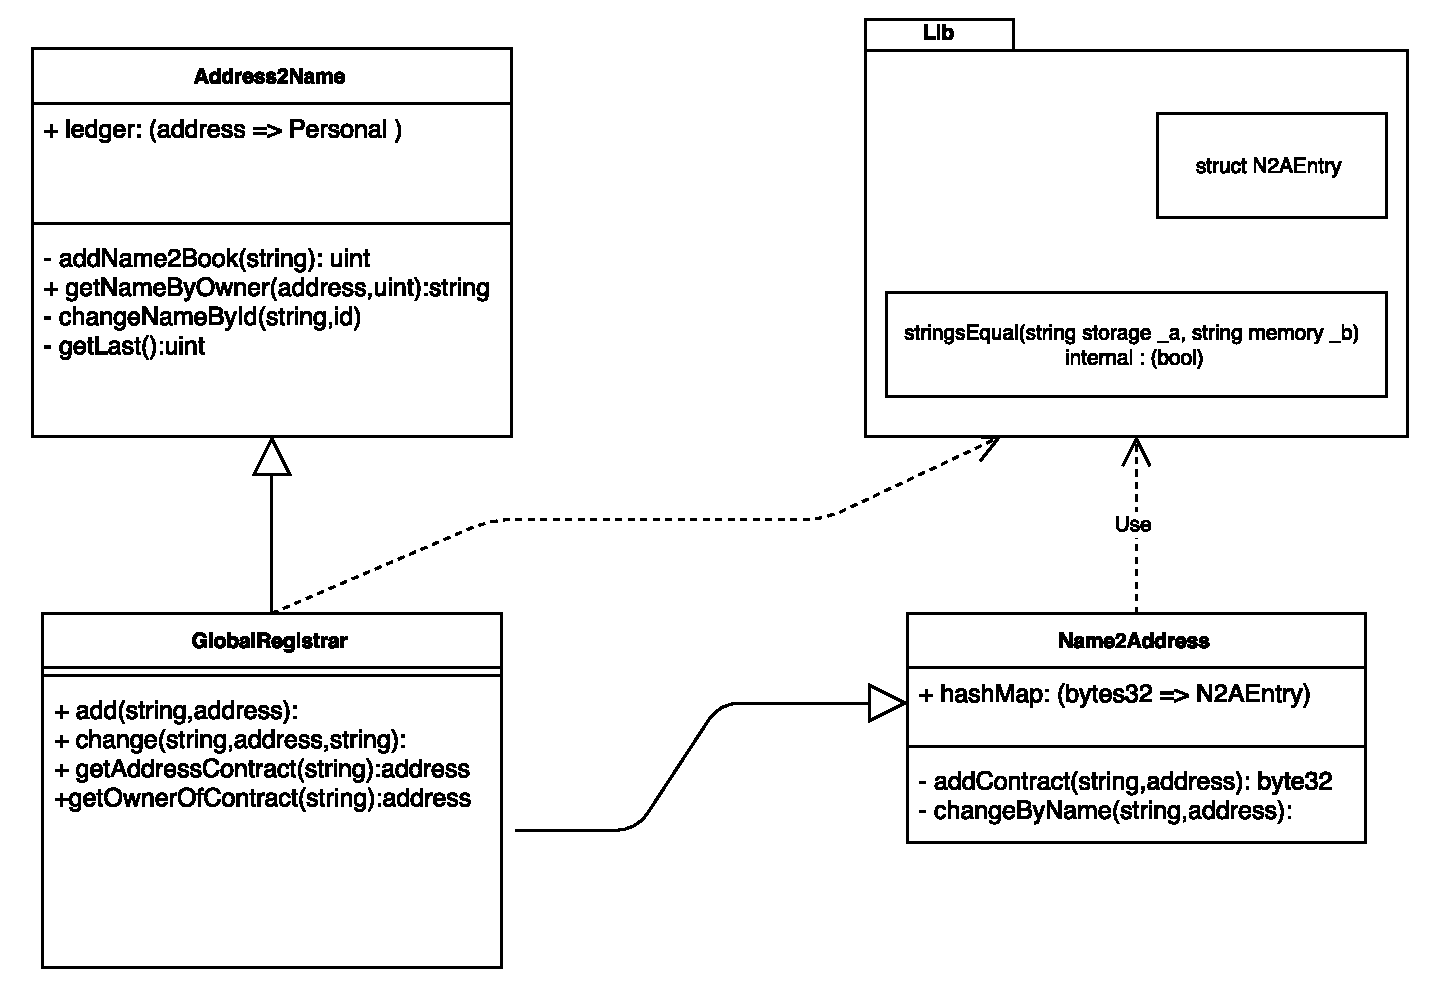
\includegraphics[width=0.75\textwidth]{GlobalRegistrar.pdf}
			\label{fig:globalregistrar}
		\end{figure}
		
	Il container \lstinline|globalRegistrar| contenuto in $GlobalRegistrar.js$ fornisce dei metodi con cui inizializzare l'istanza di un globalRegistrar, il cui codice è già caricato nella blockchain e il cui indirizzo è stato pre-caricato nel file javascript.
	
	
	
	\begin{lstlisting}
> glb = globalRegistrar.getGlobalRegistrar() 
> glb.add.sendTransaction("nomeSimbolico","0x438dfd4dfd26a42961",{from: eth.coinbase})	
	\end{lstlisting}
	
	La variabile \lstinline|glb| contiene l'istanza che collega l'abi e l'indirizzo del contratto Ethereum precedentemente caricato\footnote{Si suppone che l'utente stia lavorando connesso a una blockchain nella quale sia già stato fatto il deploy del contratto GlobalRegistrar e abbia pre-caricato l'ambiente contenente i file \lstinline|*.js|.}:
	
	Come si può vedere la registrazione della coppia di valori avviene tramite una transazione con side-effect\footnote{Consultare l'appendice \ref{appendice:b}.}.
	
	L'interrogazione del contratto, per la richiesta dell'indirizzo associato ad un nome, avviene mediante il metodo \lstinline|.getAddressContract("nomeSimbolico")|. 
	Un utente, interessato alle nuove registrazioni che vengono salvate nella blockchain, può mettersi in ascolto degli eventi lanciati dal contratto stesso \footnote{Consultare l'appendice  \ref{appendice:c} e al sotto capitolo \ref{sssec:blocco}.} che riportano dati informativi:
	
	\begin{lstlisting}
	> watcher = globalRegistrar.watchEventNewContract(glb)
	
	Nuova entry : < nomeSimbolico | 0xdfd5c578c9f5a448e71bf69cd4789211b7d94494> da l'account : 0x438dfd4dfd26a42961d878a1e27eb9f40abb0d19 .
	\end{lstlisting}

	Se due utenti vogliono registrare sotto lo stesso nome due indirizzi qualsiasi, vige il criterio \textit{first-to-file},cioè il primo arrivato acquisisce il privilegio di poter registrare e modificare l'indirizzo del nome registrato.
	Il contratto impedirà ad ogni utente di modificare record che non siano di sua proprietà e applicherà delle sanzioni nel caso venga rilevato un tentativo\footnote{Le sanzioni sfruttano i side-effect del comando throw\ref{sssec:sviluppareinsolidity}.}.

	\subsection{Digichain}
	
	Digichain è lo smart contract per la gestione delle opere autoriali. Sfruttando il contratto GlobalRegistrar gli utenti possono interagire collettivamente con il medesimo smart contract digichain semplicemente accordandosi sul suo nome simbolico.
	
	Lo smart contract consente:
	\begin{itemize}
		\item la registrazione di opere autoriali e la specifica dei metadati che la riguardano.
		\item la consultazione delle opere presenti, nonchè delle loro caratteristiche.
		\item la compravendita temporanea di opere e la verifica dello stato della cessione.
		\item la verifica della \textit{reputazione} dell'opera.
		\item la rivalsa da parte dell'autore dell'opera di rimuovere il diritto concesso al compratore in casi specifici.
	\end{itemize}
	
	Con il termine \textit{reputazione} di un opera si intende la somma di \textit{ore\_di\_utilizzo * costo\_tempo\_opera} che le persone hanno speso nell'usufruire dell'opera. Questo consentirà a tutti gli utenti di visionare la reputazione di ogni opera per scegliere quella più opportuna.
	\\

	
	Un opera è identificata tramite:
	\begin{description}
		\item[owner]: l'indirizzo del proprietario dell'opera. 
		\item[nome]: il nome dell'opera.
		\item[costoBase]: definisce in Wei l'ammontare minimo che un acquirente deve pagare per poter godere temporaneamente dell'opera.
		\item[costoTempo]: definisce in Wei il costo al minuto che un utente pagherà per usufruirne.
		\item[reputazione]: è il valore della reputazione acquisita nel corso della vita dell'opera.
	\end{description}
	
	\textbf{Registrazione}\\
	
	Un utente, allo scopo di interagire con il contratto Digichain, è obbligato a acquisire una sua istanza. Ciò si ottiene, per esempio, tramite l'istanza GlobalRegistrar nel seguente modo:
	
\begin{lstlisting}
> digichain=deployer.getIstanceFromAbiAndAddress(
	compiled.contracts["Digichain.sol:Digichain"].abi
	,glb.getAddressContract("digichain")
	)	
\end{lstlisting}
	
	Ottenuta l'istanza \lstinline|digichain|, su di essa un utente può invocare il metodo \lstinline|.creaOpera()| al quale passare i metadati dell'opera(\lstinline|(string titolo,uint256 costoBase,uint256 costoTempo)|) ed incapsulare il tutto in una transazione. 
	
	\begin{lstlisting}
	> costoBase = 200000
	> costoTempo = 10000
	> titolo = "Il titolo di questa opera"
	> digichain.creaOpera.sendTransaction(titolo, costoBase, costoTempo,{from: eth.account[0]})
	\end{lstlisting}
	
	Se la transazione è spedita correttamente\footnote{Le transazioni } ed inclusa in un blocco valido, il contratto Digichain avrà memorizzato sulla blockchain l'opera appena creata che sarà visibile a tutti tramite la call \lstinline|digichain.opere(idOpera)|.\\
	
	\textbf{Cessione del diritto}\\
	
	Ogni utente, che non sia colui che ha registrato l'opera, ha la possibilità, versando un ammontare $b$ maggiore o uguale al $costoBase$ dell'opera, di acquisire il diritto di utilizzo della stessa.

	Questo avviene attraverso i seguenti comandi:
	
\begin{lstlisting}
> bilancio = 5000000
> idOpera = 2
> digichain.compra.sendTransaction(idOpera,{from: eth.account[0],value: bilancio})
\end{lstlisting}

	Il pagamento per l'acquisto del diritto effettuato allo smart contract Digichain produrrà un nuovo contratto $R$ \textit{Registrazione} che lega l'acquirente, l'opera e l'ente di gestione delle opere Digichain. Qualsiasi operazione sul contratto $R$ appena creato potrà passare solo dalla gestione dello smart contract Digichain. 
	Se $t_0$ è il tempo di creazione del contratto $R$, indichiamo con $c$ il costo accumulato associato all'uso dell'opera nell'istante $t_1$ ed è uguale al prodotto $(t_1 - t_0) \cdot costoTempo$.
	
	Il possesso del diritto decade in due casi: se la spesa dell'utilizzo dell'opera ha superato il bilancio inizialmente versato oppure se il compratore recede dal contratto.\\
	\\
	\textbf{Recessione}\\
	
	In ogni istante, un utente che ha acquisito un diritto di utilizzo di un'opera può recedere dal contratto attraverso l'invocazione l'invio di una transazione sul metodo \lstinline|digichain.rinuncia()|. La recessione viene richiesta allo smart contract Digichain e ciò comporta la cancellazione del contratto $R$. Durante questa operazione la differenza tra il bilancio $b$ depositato in $R$ e il costo accumulato $c$ viene restituita all'utente che ha recesso, mentre, la quantità $c$ viene accreditata sul bilancio del proprietario dell'opera. Nel caso in cui il costo accumulato sia maggiore del bilancio depositato, quest'ultimo verrà interamente trasferito al creatore dell'opera.\\
	 
	%atrent forse? diagramma stati dei bilanci per rendere più chiari i movimenti nei casi in cui b>=c e b<c
	
	\textbf{Rivalsa}\\
	
	Come è stato descritto precedentemente, quando il costo accumulato supera il bilancio depositato non si scatena alcun evento\footnote{In Ethereum, come è stato osservato precedentemente, non possono essere costruiti, senza l'ausilio di sistemi (centralizzati) esterni dei meccanismi che prevedano lo scatenarsi di eventi sulla base di stati dell'esecuzione dei contratti}. Solo in questo caso specifico dove, nonostante il contratto scaduto risulti ancora registrato, il proprietario dell'opera può avvalersi del diritto di rivalsa e, e richiamando il metodo \lstinline|digichain.rinuncia()|, rimuovere personalmente il contratto sbloccando il pagamento verso di lui.\\
	

	
	Come si può vedere dalla figura \ref{fig:class-diagram} il contratto \textit{Digichain} estende la classe astratta \textit{Dao}. Questo viene fatto per dare la possibilità ad ognuno di creare la propria implementazione Digichain, anche nella previsione futura di una possibile interazione tra varie istanze Digichain specializzate in opere specifiche. L'aggregazione \textit{gestisce} mette in associazione un'istanza Digichain con $0$ o $n$ contratti Registrazione. 
	
	
			\begin{figure}
				\caption{Class diagram}
				\centering
				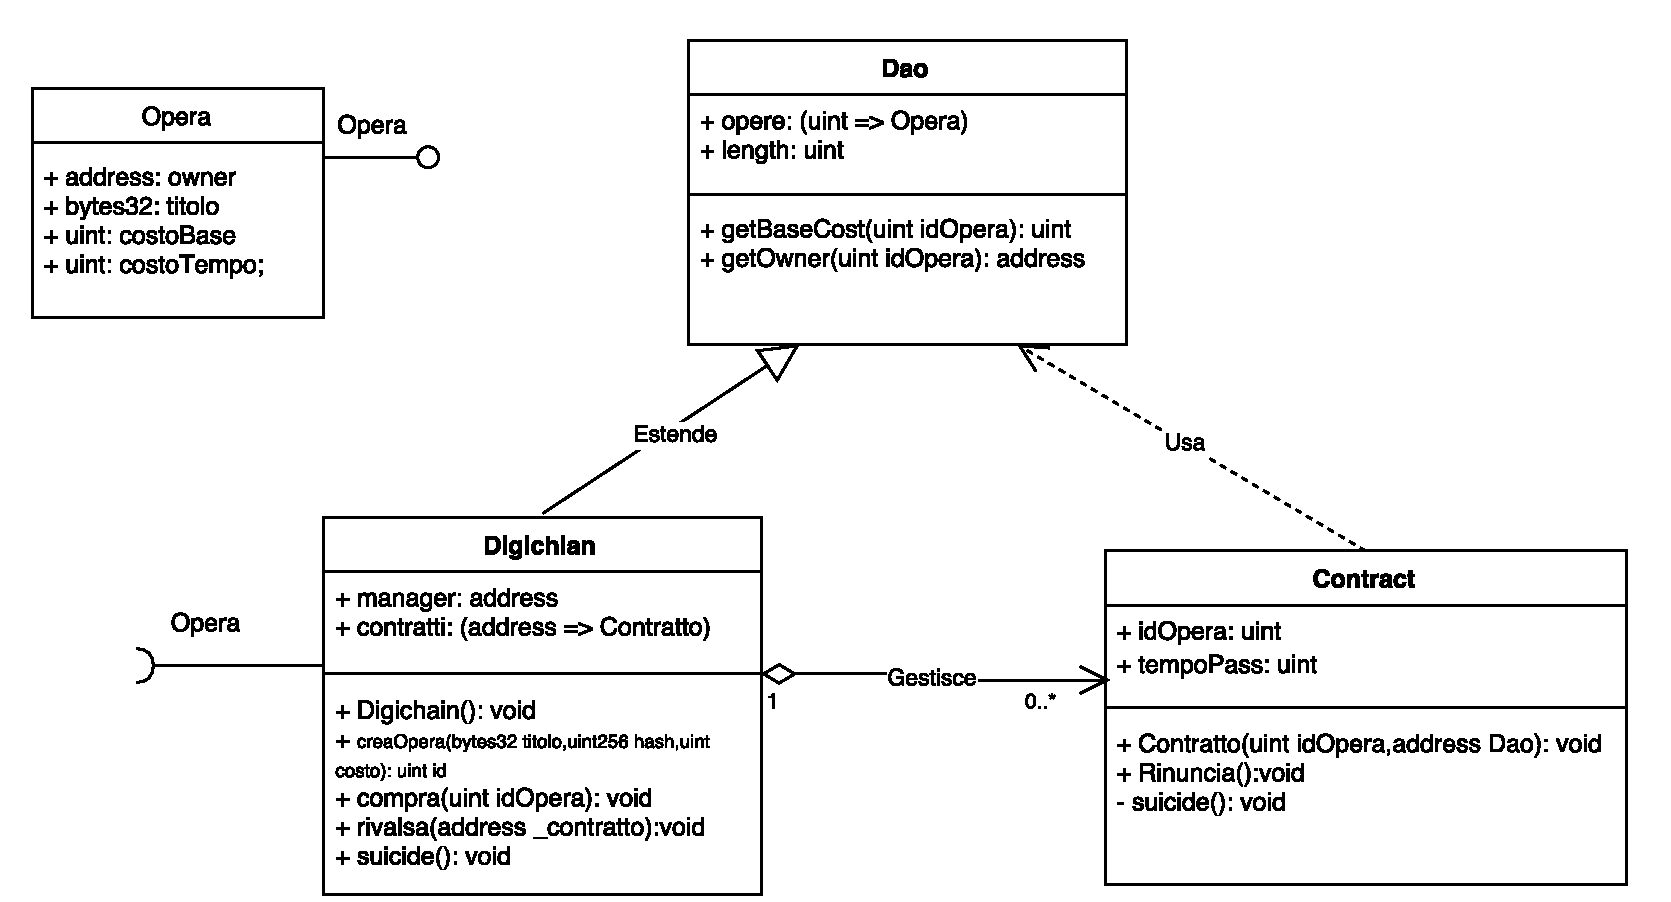
\includegraphics[width=0.75\textwidth]{class-diagram.pdf}
				\label{fig:class-diagram}
			\end{figure}
	
	
	
	\subsection{Possibili sviluppi}
	
	Ci sono diverse funzionalità che possono essere aggiunte nell'applicazione per includere nuove caratteristiche. E' possibile perseguirle con l'applicazione di pattern riguardanti i linguaggi orientati ai contratti, ma anche mediante l'utilizzo di software esterni. 
	
	\subsubsection{System of Contracts}\label{sssec:systemofcontracts}
	
	La prima interessante possibilità è l'impiego nell'applicazione del pattern \textit{System of Contracts} che consente di modificare delle componenti di una Dapp mentre essa è in esecuzione. Come già riportato più volte, gli smart contract contengono codice immutabile, l'unica operazione di modifica concessa è la cancellazione (o suicidio) del contratto. Se nelle applicazioni testate in una private-net questo aspetto può sembrare irrilevante, nelle blockchain pubbliche il deploy di contratti ha un costo. Inoltre, se la nostra applicazione distribuita ha riscosso un notevole successo e molti utenti hanno salvato dati sul suo storage, o peggio ancora all'applicazione sono stati accreditati diversi Ether, l'esecuzione del suicidio del contratto manderebbe in fumo ogni dato. 
	Quello che è possibile fare è dividere in moduli funzionali il proprio smart contract e disporre di un meccanismo che permetta l'aggiornamento del collegamento tra un'istanza di uno smart contract con un altro.
	
	In figura \ref{fig:system-of-contracts}	è possibile distinguere le classi o contratti:
	\begin{description}
		\item[Storage]: è il contratto della gestione di un'aspetto fondamentale dell'applicazione che è stato potuto isolare dal contratto Frontend e da cui esso dipende.
		\item[Frontend]: definisce la parte in comune della componente dipendente.
		\item[Registrar]: è un contratto di gestione della registrazione di record composti da nomi e indirizzi, consente al proprietario del record di poter modificare l'indirizzo a piacimento.
	\end{description}		

	\begin{figure}
		\caption{System of contracts}
		\centering
		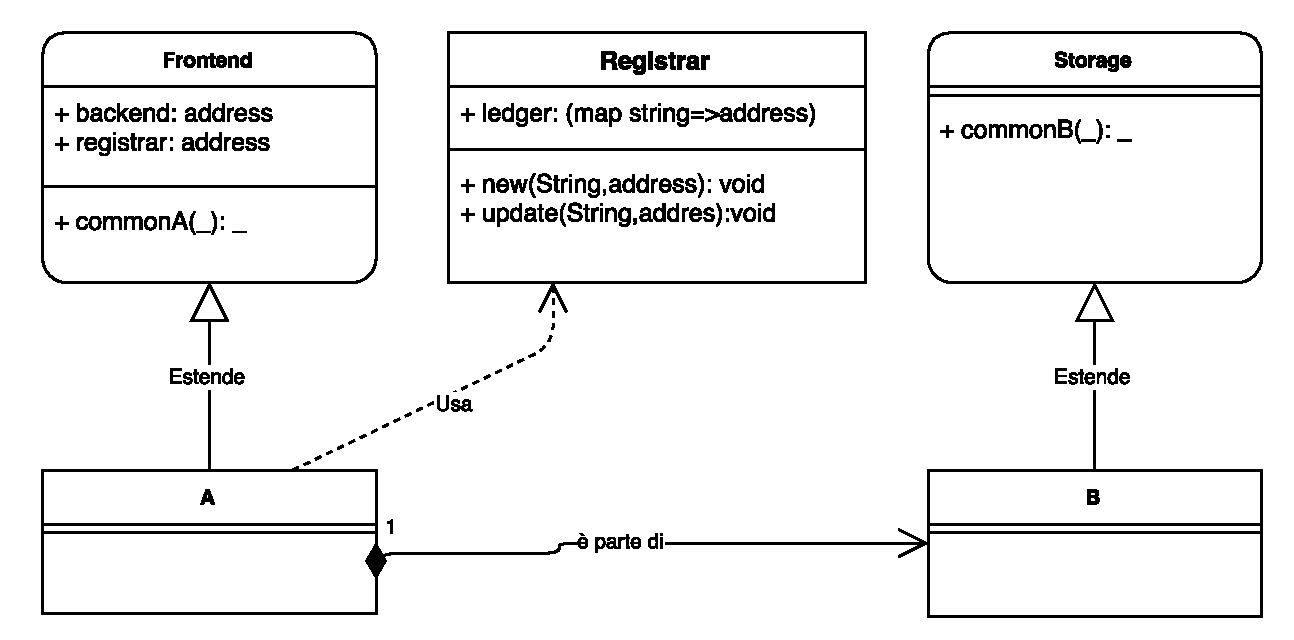
\includegraphics[width=0.75\textwidth]{System-of-contracts.pdf}
		\label{fig:system-of-contracts}
	\end{figure}

	Supponendo che il contratto Registrar è già operativo sulla blockchain, si scrive il codice per il contratto B, si esegue il deploy e l'indirizzo così ottenuto viene associato ad un nome simbolico nel contratto registrar. Viene caricato sulla blockchain il contratto A con l'indirizzo del contratto Registrar e il nome simbolico del contratto che implementa Storage.
	Nel contratto A ogni chiamata del metodo \lstinline|A.commonA()| scatena l'interrogazione del Registrar (\lstinline|registrar.ledger(backend)|) che come risultato da l'indirizzo sempre aggiornato del contratto Backend a cui deve invocare il metodo  \lstinline|commonB()|. In questo modo nel momento in cui il proprietario dell' applicazione vuole aggiornare solo la componente inclusa nel contratto B, caricherà un nuovo contratto sulla blockchain, salverà l'indirizzo di deploy nel registrar e da quel momento in poi A eseguirà il metodo del nuovo contratto.
	
	
	\subsubsection{Controlli temporizzati}\label(sssec:controllitemporizzati)
	
	Come affrontato nel sottocapitolo \ref{ssec:prolemibasatisublockchain} non esiste un meccanismo, decentralizzato ed interno alla blockchain, in Ethereum per implementare un sistema temporizzato o che reagisca ad eventi basati sullo stato dell'esecuzione dei contratti. Una frequente soluzione consiste nel fornire degli incentivi per spingere gli utenti a verificare loro stessi se si è verificato un determinato evento e impedendo che possano, allo stesso tempo, di "ingannare" il contratto per accaparrarsi l'incentivo.\\
	La funzione che, in Digichain, avrebbe bisogno di essere automatizzata è la rivalsa del contratto legata al contratto Registrazione che può trovarsi in uno stato in cui il costo $c$ accumulato nel tempo ha superato il bilancio $b$ del contratto Registrazione. La chiamata \lstinline|digichain.rivalsa(_intestatario)| è una funzione con side-effect il che comporta, anche in minima parte un costo. Questo scoraggia le persone a voler invocare la funzione, che scalerebbe degli Ether dai loro bilanci per sbloccare il pagamento verso qualcun'altro. Al contrario il controllo dell'ammontare della quantità di valuta che deve essere rimborsata viene eseguito tramite una call sullo stato del nodo locale, il che non comporta alcun costo in termini di transazioni (Si veda appendice \ref{appendice:b}). 
	
	Per aggiungere questa funzionalità e, quindi, creare degli incentivi verso gli utenti che riscuoterebbero i bilanci tramite \lstinline|.rivalsa(_intestatario)| si potrebbe aggiungere in fase di istanziazione dell'opera un nuovo valore $incentivo$ che il creatore dell'opera è disposto a pagare per il servizio di rivalsa fornito. 
	Da notare che attualmente la rivalsa è consentita solo al possessore dell'opera, ma per via della natura della funzione, incide in minima parte sul suo bilancio.
 
	


	
	
	
